\documentclass[a4paper,11pt]{article}
\pdfoutput=1 % if your are submitting a pdflatex (i.e. if you have
             % images in pdf, png or jpg format)

\usepackage{jinstpub} % for details on the use of the package, please
\usepackage{titlesec}                     % see the JINST-author-manual
\usepackage{parskip}
\usepackage{float}
\titlespacing{\section}{0pt}{\parskip}{2pt}
\titlespacing{\subsection}{0pt}{\parskip}{-\parskip}
\titlespacing{\subsubsection}{0pt}{\parskip}{-\parskip}

\title{\boldmath Detector Control System for CMS RPC at GIF++}


%% %simple case: 2 authors, same institution
 \author{Muhammad Gul, }
 \author{Michael Tytgat}
 \affiliation{Ghent University,\\Belgium}

% more complex case: 4 authors, 3 institutions, 2 footnotes
%\author[a,b,1]{F. Irst,\note{Corresponding author.}}
%\author[c]{S. Econd,}
%\author[a,2]{T. Hird\note{Also at Some University.}}
%\author[c,2]{and Fourth}

% The "\note" macro will give a warning: "Ignoring empty anchor..."
% you can safely ignore it.
% e-mail addresses: only for the forresponding author
\emailAdd{muhammad.gul@cern.ch}

\abstract{In the framework of the High Luminosity LHC upgrade program of the CMS muon system, several different RPC prototypes have been built and are now under test at the new CERN Gamma Irradiation Facility (GIF++). A dedicated Detector Control System has been developed using the WinCC-OA tool to control and monitor these prototype detectors and to store the measured parameters data.}

\keywords{Resistive-plate chambers, Detector Control System}

%\arxivnumber{1234.56789} % only if you have one

% \collaboration{\includegraphics[height=17mm]{example-image}\\[6pt]
%   XXX collaboration}
% or
\collaboration[c]{on behalf of the CMS collaboration}


% if you write for a special issue this may be useful
\proceeding{8$^{\text{th}}$ Workshop on Resistive Plate Chambers and Related Detectors\\
  February 22-26, 2016\\
  Ghent University, Belgium}

\begin{document}
\maketitle
\flushbottom

\section{Introduction}
\label{sec:intro}
The High Luminosity LHC (HL-LHC) machine will produce a higher background radiation compare to the present which will make challenges for the detectors. It is important to study the performance and stability of the current installed and future detectors in high radiation environment. Focused on these requirements, CERN Engineering- (EN) and Physics- Department (PH) made a joint project Gamma Irradiation Facility (GIF++) \cite{gif}. GIF++ is the new CERN irradiation facility located in the North Area of the CERN SPS. It is a unique place where high energy ($\sim$100 GeV) charged particles (mainly muons) are combined with a high flux of gamma radiation (662 keV) produced by 13.9 TBq $^{137}Cs$ source \cite{atlas-gif}. The attenuator system is installed to vary the gamma flux from 0 to 10$^{5}$ on the two sides of the source independently. A complete picture of GIF++ and simulation of source is shown in Fig:[\ref{gif}].\\
The CMS RPC community installed various types of RPC prototypes since April, 2015 to study the stability of detector performance for 10 years of LH-LHC. New improved RPC were also tested during the test beam of 2015. 
A dedicated control system (GIF CMS RPC) has built to control these detectors and archive the relevant parameters using WinCC-OA (PVSS) tool. The project controls High Voltage and Low Voltage modules, reading temperature, pressure and humidity both of gas and environment. The source status and attenuator values are accessed through Data Interchange Protocol (DIP), published centrally by the Engineering Department. It is a distributed project which communicates with central GIF++ project and read gas flowmeters. All these parameters are archiving in the data base (DB) and further used for trending and offline analysis.
 
\begin{figure}[htp]
\centering
\begin{tabular}{cc}
\hspace{-0.5cm}
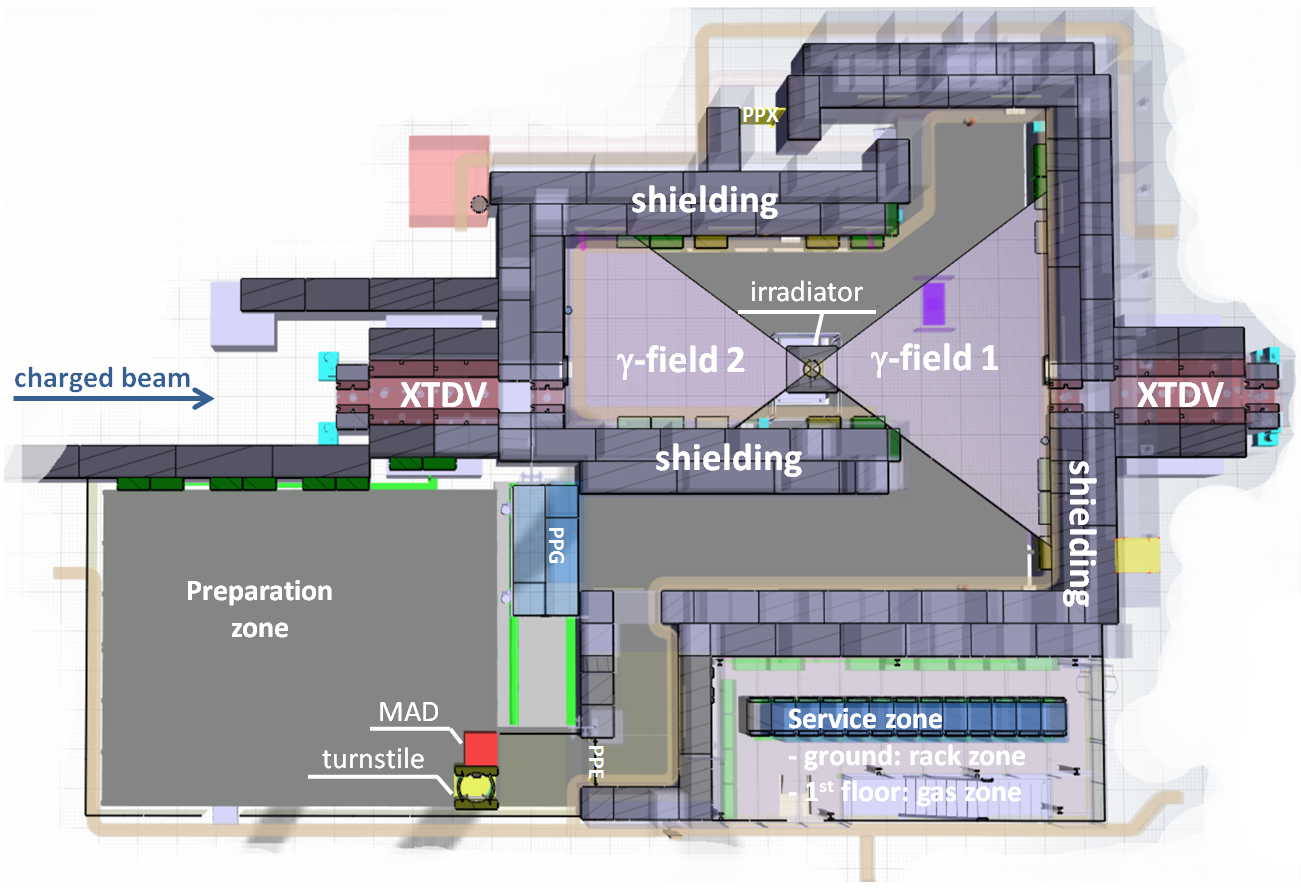
\includegraphics[scale=0.2]{images/GIF.png}
& \hspace{0.1cm} 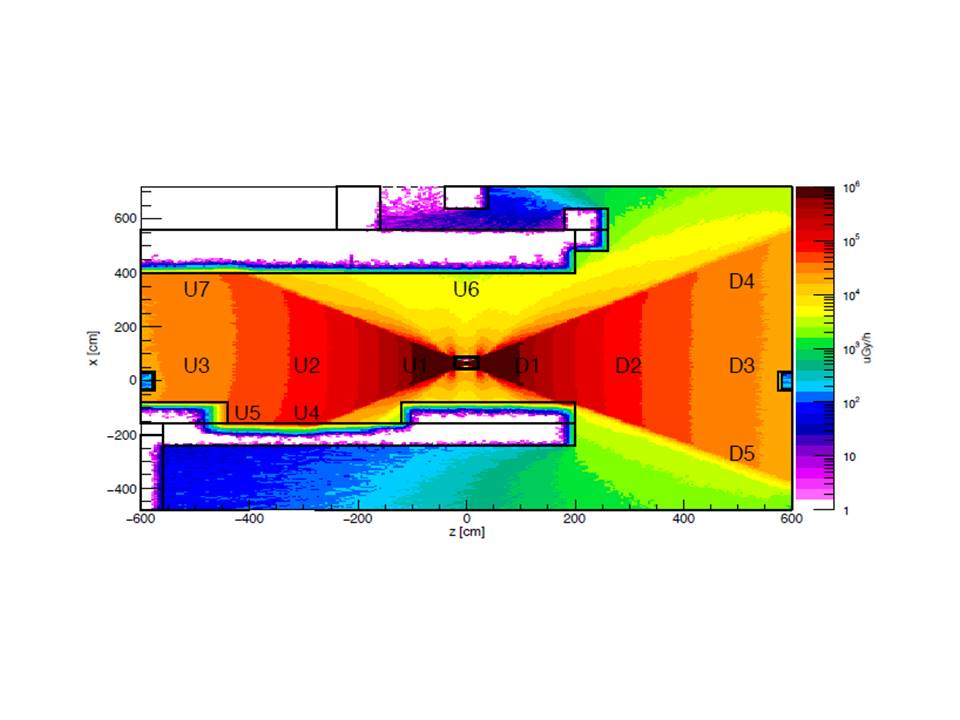
\includegraphics[scale=0.4,trim=60 130 60 130,clip]{images/simulation.jpg}\\
   $(\mathbf{a})$: GIF++ overview.\qquad\qquad&$(\mathbf{b})$: Source simulation.\\ \\
  \end{tabular}
\caption{Overview of the GIF++ and simulation of the source.}
\label{gif}
\end{figure}

\section{WinCC-OA}Large experiments at CERN use WinCC-OA as a tool to develop a control system. It has capabilities to describe a device in the form of a data point and its elements which can be used for reading and writing to corresponding device. The devices can be accessed via OPC server, ProfiBus and Drivers- make a bridge between WinCC-OA and device. Parameters of interest can be stored in the data base and used for trending and offline analysis. WinCC-OA gives a User Interface (UI) facility and access to the system using Access Control System \cite{wincc-oa}.

\section{DCS project}
The CMS RPC DCS at GIF++ has been developed by using WinCC-OA 3.11 tool, which is further equipped by the standard Joint Control Project (JCOP) framework. The JCOP framework provides extra functionalities such as the Finite State Machine (FSM), the Graphical User Interface (GUI), the alarm handler and the ORACLE data base interface \cite{g-polese}. The project controls the High Voltage and Low Voltage system through OPC protocol. The environmental and gas sensors ( for pressure, temperature and humidity) are also readable via OPC protocol. The source status and attenuator values are available centrally via Data Interchange Protocol (DIP). The project has designed as a distributed one to communicate with other projects and read valuable information. The communication has established with the central GIF++ DCS and the gases information like flow rates are readable.\\
The Finite State machine (FSM) hierarchy of the project is based on the naming convention of trolley where the detectors are installed. Each trolley has six sections and each section accommodates one detector. Currently three CMS RPCs trolleys are installed in the GIF++. Trolley 1 (RPC Consolidation) is equipped with spare RPCs, trolley 2 with small glass RPCs and trolley 3 with prototypes of improved RPCs. 
A schematic overview of DCS project is shown in Fig:[\ref{DCS_sys}]. 

\begin{figure}[htp]
\centering
\hspace{-0.5cm}
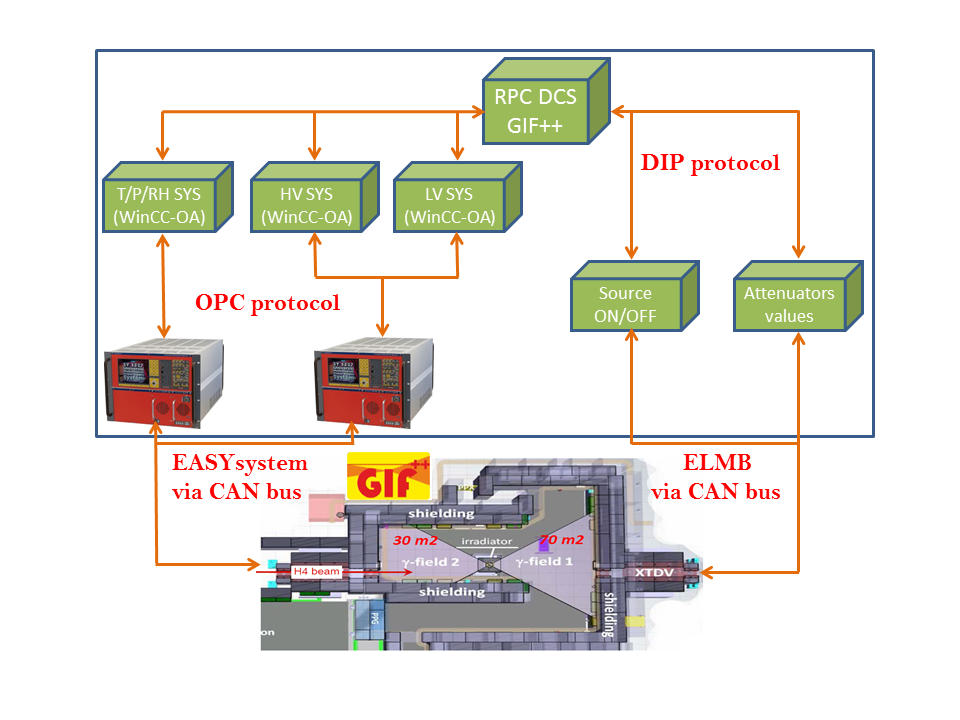
\includegraphics[scale=0.5,trim=60 30 60 30,clip]{images/DCS_sys.png}\\
 \caption{DCS project overview.}
\label{DCS_sys}
\end{figure}

 
\subsection{High and Low Voltage System}
The High and Low Voltage system is controlling and monitoring by the CAEN OPC server. Each GAP of the chamber is independently connected to a single HV channel which improves the granularity of the chamber. The LV system has divided into two types- digital and analog, where each each of them has double connection.  
\subsection{Environmental and Gas Parameters}
The performance of RPC is strongly depends on the temperature and pressure of the environment \cite{env-rpc}. Therefore it is important to measure the environmental parameters (temperature, pressure and humidity) at different locations. The applied voltage is corrected by using the environmental temperature and pressure using the formula \eqref{veff}.
\begin{equation*}\label{veff}
V_{eff} = V_{0} ( 0.2 + 0.8 (\frac{P}{P_{0}} \times \frac{T_{0}}{273+T}))
\end{equation*}
where $P_{0} = 990$ and $T_{0} = 293$.
The environmental and gas sensors (temperature, pressure and humidity) are readable through ADC (analog-to-digital converter) board which is installed in EASY crate. Under the JCOP framework, the sensors information is collected inside the sensor tree and divided further into gas and environmental sensors. The trending feature provides a comparison among different sensors located at different positions.

\subsection{High Voltage Scan and Stability Test}
The project is designed for R\&D study of detectors, most of the time high voltage scanning or stability test is running. For high voltage scanning a separate branch is made in the FSM tree where the user operate each detector independently. The stability test runs for long time and it is necessary to restart the application if it stops. Based on the requirements, a dedicated manager is running to apply the stability script and restart it automatically.    
\subsection{FSM and GUI} 
The JCOP framework provides Finite State Machine (FSM) toolkits in WinCC-OA based on SMI++. It offers an easy, robust and safe way to control the full detector through the definition of a finite number of states, transitions and actions. All the DCS hierarchy nodes are implemented through the FSM mechanism.\\
WinCC-OA provides Graphic User Interface (GUI) panel- an intuitive tool to control and monitor the detector, easy to use by non-experts and safe operation of the detector. It gives the opportunity to combine text, graphical objects and synoptic diagrams. GUI panels can be used to see the online behavior of the detector in the form of plots, tables and histograms. 

\begin{figure}[H]
\centering
\hspace{-0.50cm}
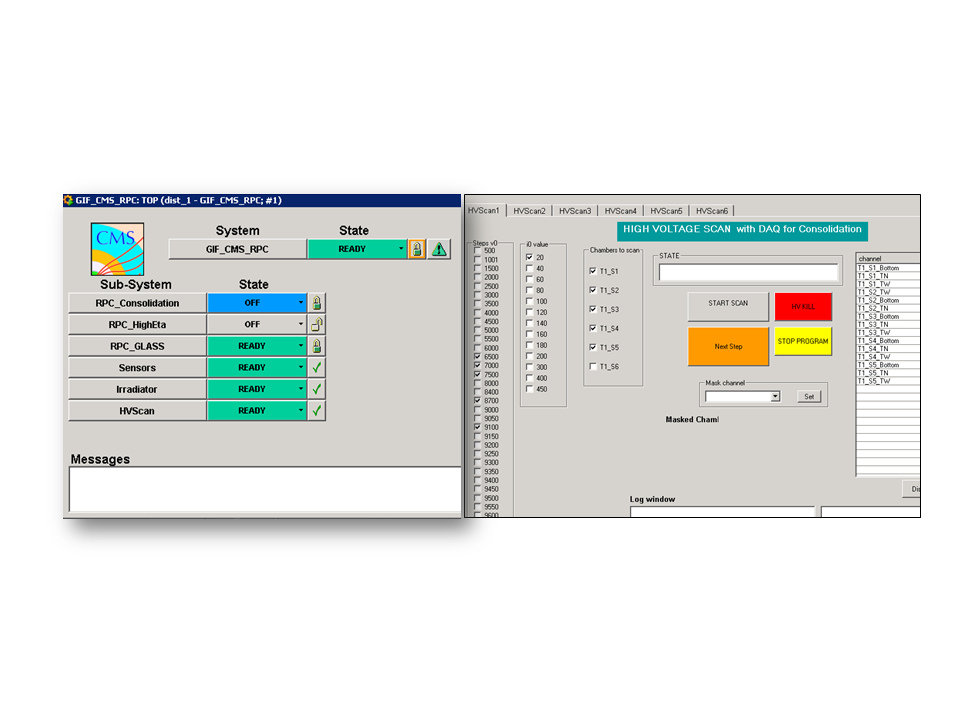
\includegraphics[scale=0.66,trim=30 150 30 140,clip]{images/GUI.png}\\
 \caption{FSM main tree and HV Scan panel using GUI.}
\label{gui}
\end{figure}

\section{Data Base}
To study the behavior of the detector over time and make offline analysis, it is necessary to store all the important parameters in a data base. WinCC-OA has its internal data base which is used in this project. The stored data is extracting within the domain of the project and using for trending and offline analysis.  

\section{Conclusion} 
The DCS project is successfully tested and applied in GIF++. Since June, 2015 the project is running in a stable state, operating the detector and archiving the data. The hardware is integrated in the project, fully controlled for High Voltage scanning and stability test. The environmental and gas sensors are included and used for T/P corrections. Gas flowmeters are reading through central DCS at GIF++ and the data are using to study the behavior of different gases. All useful parameters are archiving in the internal data base for trending and offline analysis. The project is designed for detector R\&D study, any new hardware can be included in easy and safe mode.  

\acknowledgments
Thanks to Alberto Andres Ocampo Rios and Marino Romano for their technical support to develop the project. Many thanks to Nicolas Zaganidis and Gabriella Pugliese for providing all the necessary facilities.  

% We suggest to always provide author, title and journal data:
% in short all the informations that clearly identify a document.

\begin{thebibliography}{99}
\bibitem{gif} M. R. Jakel et. al., \emph{CERN GIF++: A new irradiation facility to test large-area particle detectors for the high-luminosity LHC program},
\texttt{PoS(TIPP2014)102.} 
\bibitem{atlas-gif} B. Alvarez Gonzalez et. al., \emph{Ageing Studies on the First Resistive-MicroMeGaS Quadruplet at GIF++.}
\bibitem{wincc-oa} \href{https://wikis.web.cern.ch/wikis/display/EN/WinCC-OA+Service}{\texttt{wikis.web.cern.ch/wikis/display/EN/WinCC-OA+Service}}.
\bibitem{g-polese}G. Polese et. al., \emph{The Detector Control Systems for the CMS Resistive Plate Chamber}
\href{http://iopscience.iop.org/article/10.1088/1742-6596/219/2/022019/pdf}{\texttt{doi:10.1088/1742-6596/219/2/022019}}
\bibitem{env-rpc}Burak Bilki et. al., \emph{Environmental Dependence on the Performance of the Resistive Plate Chambers}
\href{http://iopscience.iop.org/article/10.1088/1748-0221/5/02/P02007/pdf}{\texttt{doi:10.1088/1748-0221/5/02/P02007}}

\end{thebibliography}
\end{document}
